\documentclass[10pt,a4paper]{article}

\usepackage[a4paper,top=2.75cm,bottom=4.25cm,left=2.6cm,right=2.6cm]{geometry}
\usepackage[english]{babel}
\usepackage[backend=biber,url=true,doi=true,eprint=false,style=numeric]{biblatex}
\usepackage{multicol}
\usepackage{fontspec}
\usepackage{caption}
\usepackage{etoolbox}
\usepackage{authblk}
\usepackage{titlesec}
\usepackage{tikz}
\usepackage[all]{background}
\usepackage{parskip}
\usepackage{microtype}

\setmainfont{Arial}
\setlength{\columnsep}{0.8cm}
\pagenumbering{gobble}

\addbibresource{references.bib}

\titleformat{\section}[block]{\fontsize{13pt}{15.6}\selectfont\bfseries\filcenter}{}{1em}{}
\titlespacing\section{0pt}{0cm}{0cm}

\setlength{\parskip}{0.525mm}

\newenvironment{Figure}
  {\par\smallskip\noindent\minipage{\linewidth}}
  {\endminipage\smallskip\par}

\newcommand{\SIICUSPLogo}{%
	\begin{tikzpicture}[remember picture,overlay]
		\node[anchor=north west,yshift=-2.0cm,xshift=2.9cm]%
			at (0, 0) {
\includegraphics[width=1.2cm, keepaspectratio]{imgs/siicusp_logo.png}};
	\end{tikzpicture}
}

\SetBgContents{\SIICUSPLogo}
\SetBgPosition{current page.north west}
\SetBgOpacity{1.0}
\SetBgScale{1.0}
\SetBgAngle{0.0}

\makeatletter
\patchcmd{\@maketitle}{\LARGE}{\fontsize{13pt}{15.6}\selectfont\bfseries}{}{}
\makeatother

\renewcommand\Authfont{\fontsize{13pt}{15.6}}
\renewcommand\Affilfont{\fontsize{13pt}{15.6}}

\title{AUTOMATIC LEARNING OF SUM-PRODUCT NETWORKS}
\author{\textbf{Renato Lui Geh (student), Denis Deratani Mauá (advisor)}}
\affil{Institute of Mathematics and Statistics, University of São Paulo}
\affil{\fontsize{10pt}{12}\selectfont\{renatolg,ddm\}@ime.usp.br}
\date{}

\begin{document}

\maketitle

\begin{multicols*}{2}

\section*{Objective}

Sum-product networks (SPNs) are probabilistic graphical models capable of representing probability
distributions containing a great number of variables. SPNs have shown impressive results in various
domains. Despite that, there are very few SPN inference and learning libraries currently available.
Additionaly, there hasn't been a comparative study on different SPN learning methods yet. This
project seeks to develop a free, open-source inference and learning SPN library, and to compare
three different SPN learning algorithms in the domain of image completion and classification.

%Redes soma-produto (SPN, de \textit{Sum-Product Networks}) são modelos probabilísticos que podem
%representar distribuições de probabilidade com um grande número de variáveis.  Recentemente, SPNs
%tiveram resultados impressionantes em diversas aplicações.  Apesar disso, atualmente existem poucas
%bibliotecas para inferência e aprendizado de SPNs, além de não existir nenhum estudo comparativo
%entre os diferentes métodos de aprendizado.  Este projeto busca criar uma biblioteca livre, aberta
%e gratuita para inferência e aprendizado de SPNs, além de comparar três algoritmos de aprendizado
%no domínio de classificação e compleição de imagens.

\section*{Materials and Methods}

The algorithms were implemented as part of the GoSPN\footnote{Available at:
  \url{https://github.com/RenatoGeh/gospn}} library, written in the Go programming language. The
three learning algorithms implemented were Poon-Domingos~\cite{poon-domingos},
Dennis-Ventura~\cite{clustering} and Gens-Domingos~\cite{gens-domingos}. Tests were then applied in
order to compare the performances of the three methods on the DigitsX, MNIST, Caltech-101 and
Olivetti Faces datasets.

%Os algoritmos foram implementados como parte da biblioteca GoSPN\footnote{Disponível em:
  %\url{https://github.com/RenatoGeh/gospn}} escrita na linguagem Go.  Foram implementados os
%algoritmos de aprendizado de Poon-Domingos~\cite{poon-domingos}, Dennis-Ventura~\cite{clustering} e
%Gens-Domingos~\cite{gens-domingos}. Em seguida, foram feitos testes comparando a performance dos
%três métodos nos conjuntos de dados DigitsX, MNIST, Caltech-101 e Olivetti Faces.

\section*{Results}

%Os dois algoritmos que tiveram melhores desempenhos foram o de Gens-Domingos e Dennis-Ventura. O de
%Poon-Domingos ou excedeu o limite de tempo ou memória, ou teve resultados abaixo do esperado. A
%Tabela 1 mostra a porcentagem de acerto em classificação dos dois melhores algoritmos usando 50\%
%do conjunto de dados como treino e o restante como teste.

The two methods that achieved the best performances were the Gens-Domingos and Dennis-Ventura
algorithms.  Poon-Domingos either exceeded the time or memory limit, or had unsatisfactory results.
Table 1 shows the accuracy of the two best algorithms. Tests were done by using 50\% of the dataset
as training set and the rest as test set.

\captionof*{table}{\fontsize{9pt}{10.8}\selectfont Table 1. Classification accuracy (in \%).}
\begin{tabular}{l|c|c}
  & Dennis-Ventura & Gens-Domingos\\
  \hline
  DigitsX & 99.42 & 97.14\\
  Caltech & 81.38 & 88.66\\
  Olivetti& 89.93 & 95.50\\
  MNIST   & 77.85 & 81.55\\
\end{tabular}

For the image completion task, half of the image was given as evidence to the model (represented by
the grayscale half in Figure 1) and the other half (shown in green in Figure 1) was generated by
the SPN by querying for the most probable variable valuations given the evidence. The left-hand
image was generated by the Gens-Domingos algorithm, whilst the Dennis-Ventura algorithm generated
the image on the right.

%Para a tarefa de compleição de imagem, foi dada metade da imagem como evidência para o modelo
%(visualizada na Figura 1 em escala de cinza) e gerada a outra metade (na Figura 1 em tons de
%verde) tomando as valorações mais prováveis dada evidência. A imagem da esquerda foi gerada pelo
%algoritmo de Gens-Domingos, e o da direita pelo de Dennis-Ventura.
\begin{Figure}
  \centering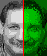
\includegraphics[scale=8.0]{imgs/gens_cmpl.png}
  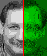
\includegraphics[scale=1.925]{imgs/dennis_cmpl.png}\\
  \vspace{-0.2cm}
  \captionof*{figure}{\fontsize{9pt}{10.8}\selectfont Figure 1. Image completion.}
\end{Figure}

\section*{Conclusions}

We achieved good classification results in different applications, such as handwritten digit
classification, object identification and face recognition. On the completion task, the algorithms
were able to identify key features, such as nose, eyes and mouth on the Olivetti dataset. The code
was documented and made available as part of the free open-source GoSPN library.

%Obteve-se bons resultados em classificação em diferentes domínios, como classificação de dígitos,
%identificação de objetos e reconhecimento de face. Em compleição, os algoritmos identificaram
%de forma razoável características como nariz, olhos e boca no conjunto Olivetti. Todo código foi
%documentado e disponibilizado de forma livre e gratuita como parte da biblioteca GoSPN\@.

\smallskip
\section*{References}
\vspace{0.1cm}

\AtNextBibliography{\fontsize{10pt}{12.0}\selectfont}
\printbibliography[heading=none]

\end{multicols*}

\end{document}
